\section{トポロジカルマップとシナリオ}
\subsubsection{トポロジカルマップ}
トポロジカルマップとは,環境をランドマークや特徴的な箇所をノードとし,その繋がりをエッジで表現した地図である.
島田らが提案したトポロジカルマップでは,ノードは通路の特徴的な箇所に配置され,エッジはノード間を接続する.
ノードにはID,通路の特徴(Type),エッジIDと相対角度(Edge)のデータが含まれ,エッジにはIDのみが含まれる.
この形式は道案内に関するアンケート結果に基づいており,人が道案内で「通路の特徴」や「向いている方向」を重視することが明らかになったことから設計された.

\begin{figure}[htbp]
  \centering
   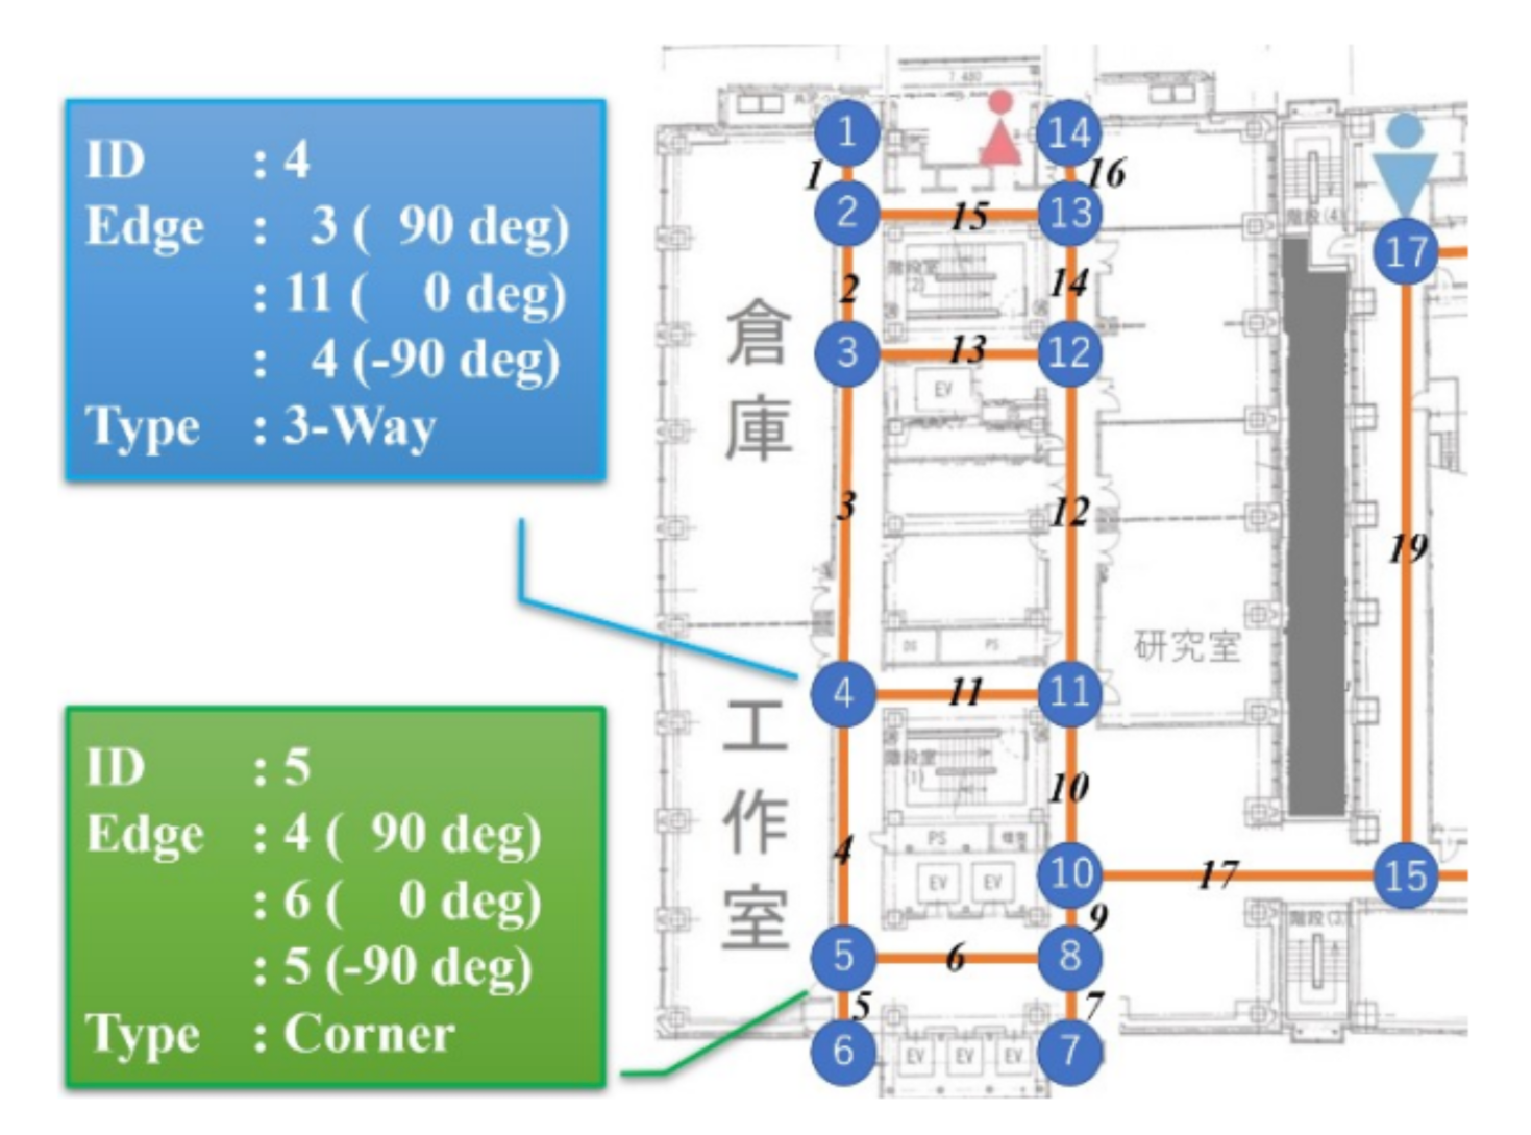
\includegraphics[width=80mm]{images/pdf/shimada/topo.pdf}
   \caption[Topological map format proposed by Shimada and others]{Topological map format proposed by Shimada and others(Quoted from\cite{shimada2020})}
   \label{fig:topo}
\end{figure}

\clearpage
\subsubsection{シナリオ}
シナリオは,トポロジカルマップ上の目的地までの経路を「条件」と「行動」の組み合わせで表現する手法である.
「条件」は「次の角」や「突き当たりまで」などを指し,「行動」は「直進」や「右折」などを指す.
この形式はトポロジカルマップ同様に道案内に関するアンケート結果に基づいており,人が「条件」と「行動」を組み合わせて道案内をすることが明らかになったことから設計された.
例として,特定の経路はと表現される.

\begin{figure}[htbp]
  \centering
   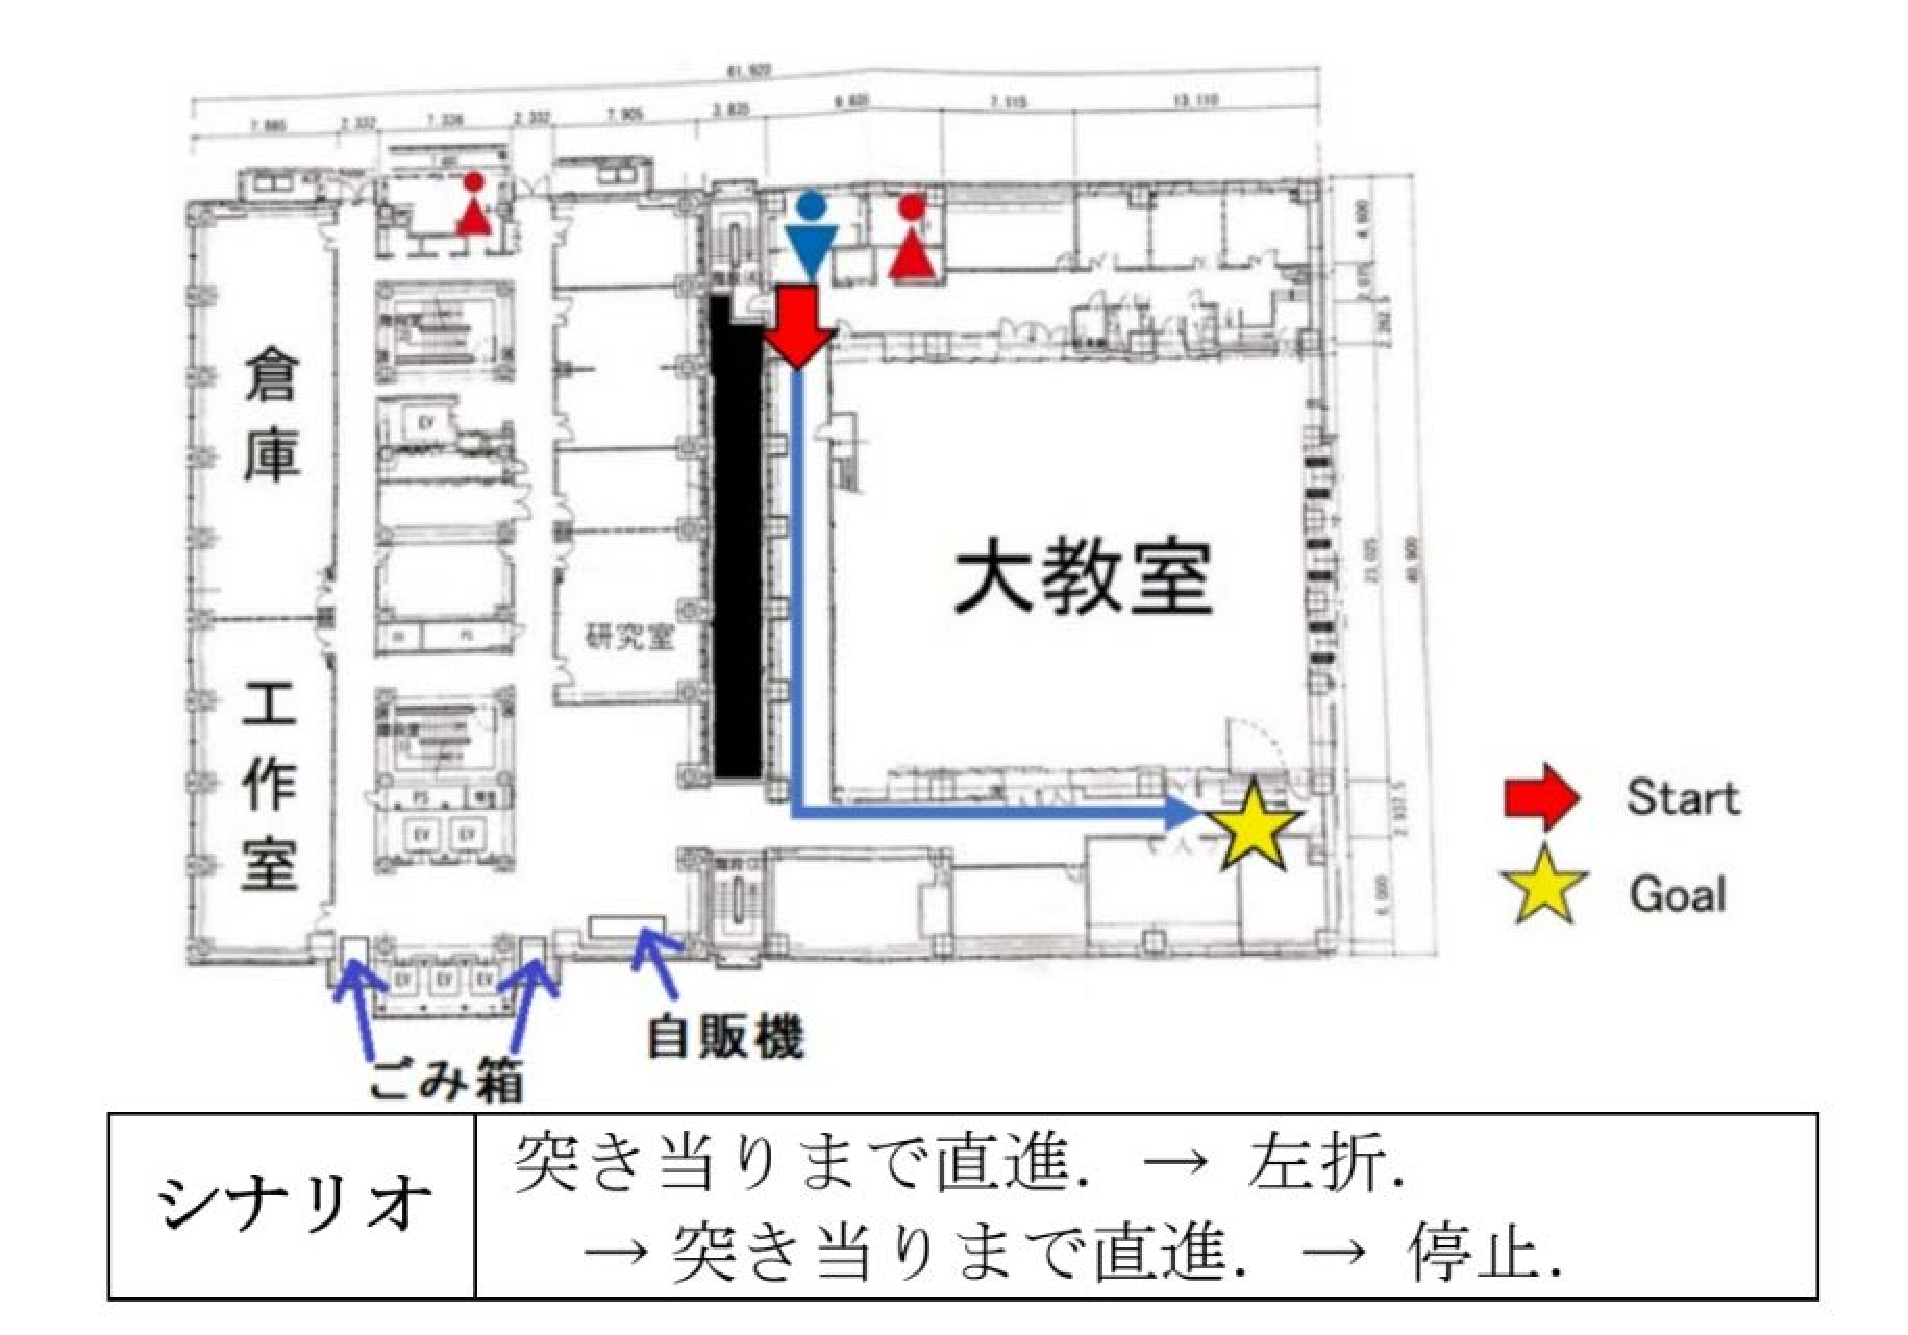
\includegraphics[width=90mm]{images/pdf/shimada/scenario.pdf}
   \caption{Topological map format proposed by Shimada and others(Quoted from\cite{shimada2020})}
   \label{fig:topo}
\end{figure}